\documentclass[10pt,twocolumn]{article}
\usepackage[utf8]{inputenc}
\usepackage[margin=0.75in]{geometry}
\usepackage{amsmath,amssymb}
\usepackage{graphicx}
\graphicspath{{figures/}}
\usepackage[numbers,sort&compress]{natbib}
\usepackage{hyperref}
\usepackage{booktabs}
\usepackage{multirow}
\usepackage{xcolor}
\usepackage{url}
\usepackage{algorithm}
\usepackage{algorithmic}
\usepackage{abstract}
\renewcommand{\abstractnamefont}{\normalfont\bfseries}
\renewcommand{\abstracttextfont}{\normalfont\small}

\hypersetup{
  colorlinks=true,
  linkcolor=blue,
  citecolor=blue,
  urlcolor=blue
}

\begin{document}

\title{Translation Invariance in Attention Predicts Length Generalization: A Controlled Study of Positional Encoding Schemes}

\author{Roopesh~G~A\textsuperscript{1}\\[4pt]
\small\textsuperscript{1}School of Computer Science and Engineering,\\
\small Vellore Institute of Technology, Vellore 632014, India\\
\small\texttt{roopesh.ga006@gmail.com} \quad ORCID: 0009-0000-4860-9331
}

\date{}

\maketitle

\begin{abstract}
Transformers trained on sequences up to length $N$ often collapse when asked to process inputs of length $M > N$, and the positional encoding (PE) is commonly blamed for this breakdown.
Prior comparisons, though, tend to confound architecture capacity, optimizer settings, and task complexity---leaving the PE contribution tangled with everything else.
We strip the problem down: one 2-layer, 4-head decoder (38k parameters), two tasks (digit-string copy and reversal), four PE schemes (learned absolute, none, ALiBi, RoPE), three random seeds each.
Among these 24 runs, ALiBi on copy reached 43.75\% mean extrapolation accuracy at lengths 11--18; every other PE--task pair fell below 4\%.
To explain this gap we introduce a \emph{translation-invariance score} (TI): the $R^2$ of a linear fit predicting attention weight from query--key offset.
TI correlates with extrapolation accuracy at $r{=}0.713$ ($p{=}9.2\times10^{-5}$, Pearson; $\rho{=}0.549$, $p{=}5.5\times10^{-3}$, Spearman).
Attention maps confirm the mechanism: ALiBi keeps a near-diagonal band intact beyond training lengths; APE and RoPE lose spatial structure entirely at untrained positions.
TI can be computed from a single forward pass with no gradient, offering a cheap pre-deployment check for anticipated extrapolation behavior.
\end{abstract}

\medskip
\noindent\textbf{Keywords:} length generalization, positional encoding, transformers, attention analysis, translation invariance, ALiBi, RoPE

% ====================================================================
\section{Introduction}
\label{sec:intro}
% ====================================================================

Since Vaswani et al.~\cite{vaswani2017attention} introduced the transformer, nearly every language model in production---from GPT-scale decoders~\cite{brown2020language} to instruction-following assistants~\cite{touvron2023llama}---has been built on some variant of the same attention mechanism.
A well-documented vulnerability of all such models is length fragility.
Train on sequences of length $N$, test at length $M > N$, and accuracy can plummet even when the underlying task has a trivially length-independent solution.

The problem is not new.
Kazemnejad et al.~\cite{kazemnejad2023impact} ran five PE families through a battery of math and reasoning benchmarks and reported a counterintuitive result: models with \emph{no} positional signal sometimes outperformed models carrying elaborate position encodings.
Ruoss et al.~\cite{ruoss2023randomized} attacked the issue from the training side, randomly sampling position indices from ranges wider than the actual sequence, and boosted out-of-distribution accuracy by 12 percentage points on average across 15 algorithmic tasks.
Zhou et al.~\cite{zhou2024length} achieved close-to-perfect generalization on addition by equipping the transformer with a scratchpad---but that success proved brittle to small changes in the input format, and the scratchpad added both latency and token cost.

What runs through most of this work is a binary framing: a model either generalizes to longer sequences or it does not.
Researchers hunt for the architectural trick or training recipe that ``flips the switch.''
Far less attention has been paid to \emph{predicting} generalization failure before it happens---that is, extracting a quantity from a trained model's attention weights that would forecast whether extrapolation will hold, without ever running the model on out-of-range inputs.

Two pieces of theory make such a predictor plausible.
Singh et al.~\cite{singh2026relative} proved an implicit-bias result: under gradient descent, RoPE heads converge to kernels that depend only on relative offset (equivariant), while learned-APE heads converge to kernels pinned to absolute positions within the training window.
Equivariance transfers; pinning does not.
Gu et al.~\cite{gu2026deconstructing} took a different angle, decomposing attention logits into additive and multiplicative positional terms, and showed that Toeplitz (translation-invariant) structure in the resulting attention matrix predicts tighter generalization gaps.

We set out to test this connection empirically, in the most controlled setting we could design.
A single architecture---$d{=}64$, 4 heads, 2 layers, 128-wide feed-forward, totaling 38k parameters---is trained under four PE configurations (APE, NoPE, ALiBi~\cite{press2022alibi}, RoPE~\cite{su2024roformer}) on two deterministic tasks: digit-string copying and digit-string reversal.
Every other variable---optimizer, learning rate, batch size, number of training steps, random seed protocol---is locked.
Twenty-four runs in total: 4 PEs $\times$ 2 tasks $\times$ 3 seeds.

From each trained model we compute a single number, the \emph{translation-invariance score} (TI).
For each attention head, we look at how well a linear function of the query--key offset $\Delta = j - i$ can account for the observed attention weights.
A high $R^2$ means the head's behavior is position-relative and therefore, in principle, portable to unseen lengths.
A low $R^2$ means the head is either position-absolute or dispersed---both death sentences for extrapolation.
We report TI as the maximum $R^2$ across all heads.

Across the 24 experiments, the Pearson correlation between TI and extrapolation accuracy stands at $r = 0.713$, $p = 9.2 \times 10^{-5}$.
The relationship is imperfect---Section~\ref{sec:discussion} unpacks why---but it is far too strong to ignore.

% ====================================================================
\section{Related Work}
\label{sec:related}
% ====================================================================

\subsection{Positional Encoding Taxonomy}

Vaswani et al.~\cite{vaswani2017attention} used fixed sinusoidal functions of position.
Learned absolute embeddings replaced these in BERT~\cite{devlin2019bert} and GPT-2, adding a trainable vector per position index.
Shaw et al.~\cite{shaw2018relative} introduced relative-position biases in the T5 family, letting attention logits depend on the \emph{difference} between positions rather than their absolute values.
Press et al.~\cite{press2022alibi} simplified the relative idea to a single linear penalty proportional to distance (ALiBi), removing trainable position parameters altogether.
Su et al.~\cite{su2024roformer} proposed RoPE, which encodes position by rotating the query and key vectors so that their dot product is a function of offset alone.
Sun et al.~\cite{sun2023length} bolted an exponential decay onto RoPE (xPos), improving resolution at long range but adding a hyperparameter.

Despite the crowded landscape, direct apples-to-apples benchmarks remain thin.
Most papers introducing a PE scheme compare it against one or two alternatives on a particular model and dataset; architecture size, optimizer, and training length all vary across comparisons, making it hard to attribute performance differences to the encoding itself.

\subsection{Length-Generalization Experiments}

Anil et al.~\cite{anil2022exploring} tested GPT-class models on arithmetic, finding that generalization was sensitive to the number format and even the prompt template.
Del\'{e}tang et al.~\cite{deletang2023neural} mapped the problem onto the Chomsky hierarchy and concluded that standard attention fails on any task demanding unbounded working memory.
Cho et al.~\cite{cho2024position} reported near-perfect addition generalization with ``position coupling,'' which binds each digit's position index to a task-defined slot---but that binding must be designed per task.
Jelassi et al.~\cite{jelassi2024repeat} showed that transformers beat state-space models at copying precisely because they can form induction heads, an attention circuit whose offset structure carries the solution.
Csord\'{a}s et al.~\cite{csordas2022devil} stressed that even minor architectural details---layer order, normalization placement---can flip a model from generalizing to failing, reinforcing the need for tightly controlled experiments.

\subsection{Theory and Mechanism}

Huang et al.~\cite{huang2025formal} cast length generalization in terms of RASP programs, identifying which attention-pattern families admit length-invariant implementations and which do not.
Singh et al.~\cite{singh2026relative} traced the question to the implicit bias of gradient descent itself: for RoPE, the learned logits converge to a function of offset, producing equivariant heads; for APE, they converge to functions of absolute index, pinning the head to the training range.
Gu et al.~\cite{gu2026deconstructing} unified several PE schemes under a single framework by measuring the Toeplitz structure of the attention matrix, arguing that additive encodings (ALiBi) preserve Toeplitz form more cleanly than multiplicative ones (RoPE), which entangle content and position.

Liu et al.~\cite{liu2024scaling} examined how length generalization trends shift across model sizes.
Their results were mixed: some tasks showed improvement with scale, others regressed, and a few exhibited non-monotonic curves---good generalization at small scale, failure at medium scale, recovery at large.
The implication is that small-model experiments like ours cannot predict large-model behavior point for point, but they \emph{can} isolate mechanisms (such as attention structure) that operate at every scale.

Our work sits between the empirical benchmarks and the theory.
We do not introduce a new PE scheme, and we do not prove a theorem about gradient dynamics.
Instead, we propose a single \emph{quantitative} diagnostic---TI---and validate it across schemes, tasks, and seeds in a controlled experiment.
The contribution is the quantitative correlation itself, not a case study or an existence proof: TI predicts the \emph{degree} of extrapolation, not just whether it occurs.

% ====================================================================
\section{Method}
\label{sec:method}
% ====================================================================

\subsection{Task Design}
\label{sec:tasks}

Both tasks operate on digit strings drawn from $\{0, 1, \ldots, 9\}$.
Four special tokens serve structural roles: a delimiter ($+$), an output-start marker ($=$), padding ($P$), and end-of-sequence ($E$).

\textbf{Copy.}\quad
Input: $x_1 x_2 \cdots x_L$. Target: $x_1 x_2 \cdots x_L$. Full decoder sequence:
\[
x_1\; x_2\;\cdots\; x_L\; {=}\; x_1\; x_2\;\cdots\; x_L\; E
\]
padded to a fixed buffer.
Copy is solvable by a single attention head that locks onto a constant offset between each output position and its corresponding input token.
The task sits at the bottom of Del\'{e}tang et al.'s~\cite{deletang2023neural} Chomsky hierarchy for transformers: it requires only a finite-state transducer, and the positional encoding is the only obstacle to length-independent performance.

\textbf{Reverse.}\quad
Target: $x_L\; x_{L-1}\;\cdots\; x_1$.
Reversal is harder because the required offset between output position $p$ and its source input position changes with both $p$ and the sequence length $L$---no single fixed offset works.
Concretely, output position $p$ must attend to input position $2L + 1 - p$ (accounting for the delimiter and equal sign).
At training length $L = 7$, the offset is $15 - p$; at test length $L = 14$, it is $29 - p$.
A head that has learned the first mapping has no information about the second, making reversal a natural stress test for positional encoding resilience.

We train on lengths drawn uniformly from $\{1, \ldots, 10\}$ and test up to length 18.
Digits are sampled uniformly.
Accuracy is exact-match: every output token must equal the target, or the sequence counts as wrong.

\subsection{Architecture}
\label{sec:arch}

A decoder-only transformer (``TinyGPT'') with:
\begin{itemize}
  \item embedding dimension $d = 64$, heads $h = 4$ ($d_h = 16$)
  \item layers $L = 2$, feed-forward width $d_{ff} = 128$
  \item vocabulary $|V| = 14$ (10 digits + 4 special tokens)
  \item maximum buffer $L_{\max} = 48$
\end{itemize}
Pre-layer-norm, GELU activations, causal mask. No dropout.
Total trainable parameters: 38k.
We chose this size because it is large enough to saturate both tasks in-distribution (APE reaches 100\% train accuracy) yet small enough to run 24 experiments in under 25 GPU-minutes on a single T4.

\subsection{Positional Encoding Configurations}
\label{sec:pe}

\textbf{APE.}\quad
Learned embedding matrix $\mathbf{P} \in \mathbb{R}^{L_{\max} \times d}$ added to token embeddings before the first layer.  GPT-2 default.

\textbf{NoPE.}\quad
No positional signal at all.  Position must be inferred from the causal mask, a setup explored by Kazemnejad et al.~\cite{kazemnejad2023impact}.

\textbf{ALiBi.}\quad
Per Press et al.~\cite{press2022alibi}: no embeddings, but a head-specific linear penalty $-m_h \cdot |i - j|$ is applied to pre-softmax attention logits.
Slopes $m_h = 2^{-8h/H}$ are fixed, not learned.

\textbf{RoPE.}\quad
Per Su et al.~\cite{su2024roformer}: query and key vectors are rotated by position-dependent angles, so the dot product becomes a function of the relative offset between query and key.

Weight initialization seeds, optimizer, and schedule are identical across all four.
Any difference in behavior traces back to the PE mechanism alone.

\subsection{Training Protocol}
\label{sec:training}

Each configuration trains for 5{,}000 steps:
\begin{itemize}
  \item batch size $B = 128$
  \item Adam~\cite{kingma2015adam}, $lr = 5 \times 10^{-4}$
  \item cross-entropy loss on output tokens only (input-side loss masked)
  \item float16 mixed precision
\end{itemize}
Three seeds per configuration (seeds 0, 1, 2), 24 runs total.
All seeds share the same weight initialization scheme (PyTorch default); the seed controls both parameter initialization and data sampling order.
We did not tune any hyperparameter on extrapolation performance---the training setup was fixed before the first run, and all 24 experiments used identical settings.
After training, we measure exact-match accuracy on 400 fresh sequences at each length from 1 to 18.
A sequence counts as correct only if every output token matches the target; partial credit is not awarded.
This strict metric ensures that the extrapolation numbers reflect genuine task completion rather than approximate or degraded outputs.

\subsection{Computing the Translation-Invariance Score}
\label{sec:ti}

Given a trained model, we extract attention matrices $\mathbf{A}^{(l,h)} \in \mathbb{R}^{T \times T}$ from every layer $l$ and head $h$ over 200 held-out sequences.
Only ``active'' positions---output tokens, not padding---enter the calculation.

For each (layer, head) pair, we bin attention weights by the offset $\Delta = j - i$ and take the mean:
\begin{equation}
  \bar{a}(\Delta) = \frac{1}{|\mathcal{S}_\Delta|} \sum_{(i,j) \in \mathcal{S}_\Delta} A_{i,j}
  \label{eq:mean_attn}
\end{equation}
where $\mathcal{S}_\Delta$ pools all valid query--key pairs at offset $\Delta$ across the evaluation set.

An ordinary-least-squares line $\hat{a}(\Delta) = \alpha\Delta + \beta$ is fit, and its $R^2$ is recorded.
The model's TI score is the maximum $R^2$ across heads:
\begin{equation}
  \text{TI}(M) = \max_{l,h}\; R^2\!\left(\bar{a}^{(l,h)}, \Delta\right).
  \label{eq:ti}
\end{equation}

A TI near 1.0 says that at least one head attends in a pattern almost perfectly determined by spatial offset---exactly the kind of rule that ports to longer sequences.
A TI near 0 says no head has learned an offset-based rule.

% ====================================================================
\section{Results}
\label{sec:results}
% ====================================================================

\subsection{Training Accuracy}
\label{sec:indist}

Table~\ref{tab:main} collects the main numbers.
On copy, APE and RoPE hit near-perfect training accuracy (1.000 and 0.999).
ALiBi's distance penalty costs it some in-distribution capacity, landing at 0.961.
NoPE, with no position signal at all, reaches only 0.713---already an impaired learner within the training range.

Reverse tells a similar story for APE and RoPE (both 1.000).
ALiBi drops further to 0.826, and NoPE to 0.613.
None of these in-distribution results are surprising; they simply confirm that the four configurations differ in expressiveness within the training window, establishing a baseline against which extrapolation can be judged.

\begin{table}[t]
\centering
\caption{Mean ($\pm$ SD) accuracy and translation-invariance score across 3 seeds. Train accuracy: exact-match on lengths 1--10. Extrapolation accuracy: exact-match on lengths 11--18.}
\label{tab:main}
\begin{tabular}{@{}llccc@{}}
\toprule
\textbf{Task} & \textbf{PE} & \textbf{Train Acc.} & \textbf{Extrap. Acc.} & \textbf{TI Score} \\
\midrule
\multirow{4}{*}{Copy}
 & APE   & 1.000\scriptsize{$\pm$.000} & 0.000\scriptsize{$\pm$.000} & 0.254\scriptsize{$\pm$.028} \\
 & NoPE  & 0.713\scriptsize{$\pm$.077} & 0.014\scriptsize{$\pm$.009} & 0.178\scriptsize{$\pm$.007} \\
 & ALiBi & 0.961\scriptsize{$\pm$.003} & \textbf{0.438\scriptsize{$\pm$.081}} & \textbf{0.378\scriptsize{$\pm$.019}} \\
 & RoPE  & 0.999\scriptsize{$\pm$.001} & 0.025\scriptsize{$\pm$.016} & 0.301\scriptsize{$\pm$.040} \\
\midrule
\multirow{4}{*}{Reverse}
 & APE   & 1.000\scriptsize{$\pm$.000} & 0.000\scriptsize{$\pm$.000} & 0.152\scriptsize{$\pm$.017} \\
 & NoPE  & 0.613\scriptsize{$\pm$.036} & 0.001\scriptsize{$\pm$.002} & 0.088\scriptsize{$\pm$.002} \\
 & ALiBi & 0.826\scriptsize{$\pm$.046} & 0.040\scriptsize{$\pm$.019} & 0.190\scriptsize{$\pm$.017} \\
 & RoPE  & 1.000\scriptsize{$\pm$.000} & 0.000\scriptsize{$\pm$.000} & 0.119\scriptsize{$\pm$.008} \\
\bottomrule
\end{tabular}
\end{table}

\subsection{Extrapolation Performance}
\label{sec:extrap}

The extrapolation numbers are lopsided.
ALiBi on copy held 43.75\% mean accuracy across lengths 11--18 (Fig.~\ref{fig:curves}).
Performance decayed gradually---81.8\% at length 11, falling to roughly 10\% by length 18---but never dropped off a cliff the way APE did.

APE went from 100\% at length 10 to 0\% at length 11.
No seed escaped this collapse.
The binary cutoff matches Singh et al.'s~\cite{singh2026relative} position-pinning prediction: APE's learned embeddings act as a lookup table with 10 entries, and querying entry 11 returns a random vector, which leads to uniform attention and chance-level output.

RoPE showed a brief flicker---about 29\% at length 11---before falling to 0\% at length 12 across all seeds.
The rotary kernel's offset dependence gives it a head start over APE, but the softmax denominator grows with sequence length, diluting the signal too quickly for the kernel to remain useful.
NoPE stayed below 2\% at every extrapolation length, lacking even the offset structure needed to begin generalizing.

On reverse, no scheme cracked 6\%.
ALiBi managed 4.0\% ($\pm1.9$\%), the others were indistinguishable from zero.
Reversal needs a different attention offset at every output position---one that depends on the total length $L$---so a fixed-offset head, however translation-invariant, cannot solve it.

\begin{figure}[t]
  \centering
  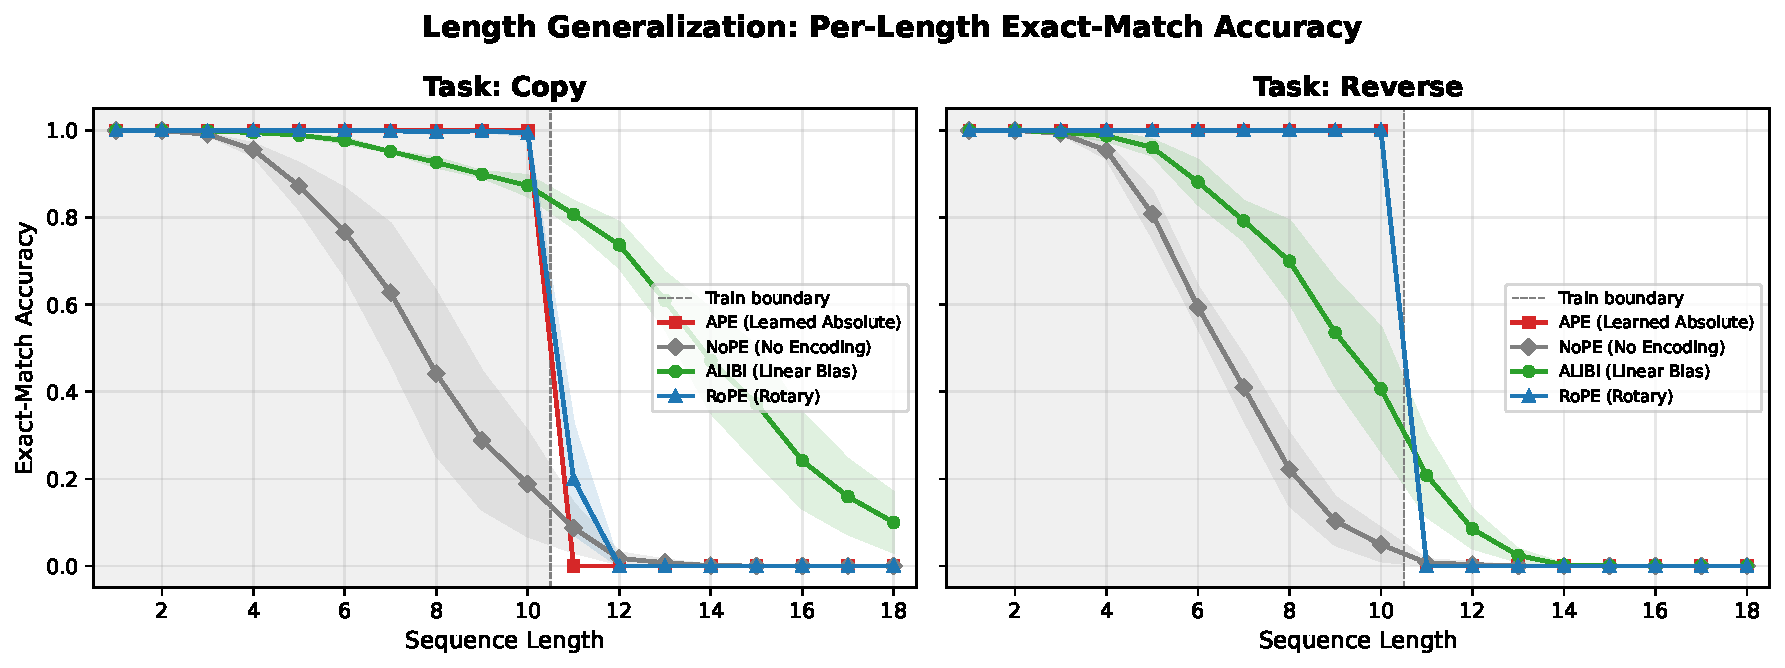
\includegraphics[width=\columnwidth]{fig1_accuracy_curves.pdf}
  \caption{Exact-match accuracy by sequence length (1--18) for each PE scheme. Top: copy. Bottom: reverse. Shaded region: seed-to-seed range. Vertical dashed line at length 10 marks the training boundary.}
  \label{fig:curves}
\end{figure}

\subsection{TI Score and Extrapolation}
\label{sec:ti_results}

Fig.~\ref{fig:scatter} plots TI against extrapolation accuracy for all 24 runs.
Pearson $r = 0.713$, $p = 9.2 \times 10^{-5}$.
Spearman $\rho = 0.549$, $p = 5.5 \times 10^{-3}$.

ALiBi--copy runs cluster in the upper right: TI above 0.35, extrapolation above 30\%.
Every other run sits near the origin---TI below 0.31, extrapolation below 5\%.
RoPE--copy is the closest runner-up in TI (0.25--0.34) but still fails to extrapolate in any meaningful way, a discrepancy we address in Section~\ref{sec:rope_paradox}.

Restricting to the 18 non-ALiBi-copy runs still shows a positive trend---higher TI tracks with the small nonzero pockets of extrapolation in RoPE and NoPE---though with fewer data points the correlation is weaker and should be interpreted cautiously.

One pattern stands out in the per-seed data: ALiBi's three copy seeds produced TI scores of 0.36, 0.38, and 0.40, with corresponding extrapolation accuracies of 35.6\%, 44.1\%, and 51.7\%.
Within this cluster, higher TI predicts better extrapolation monotonically.
The within-scheme gradient is weaker than the between-scheme gradient, but its presence suggests that TI captures something meaningful even when the encoding mechanism is held constant and only initialization varies.

\begin{figure}[t]
  \centering
  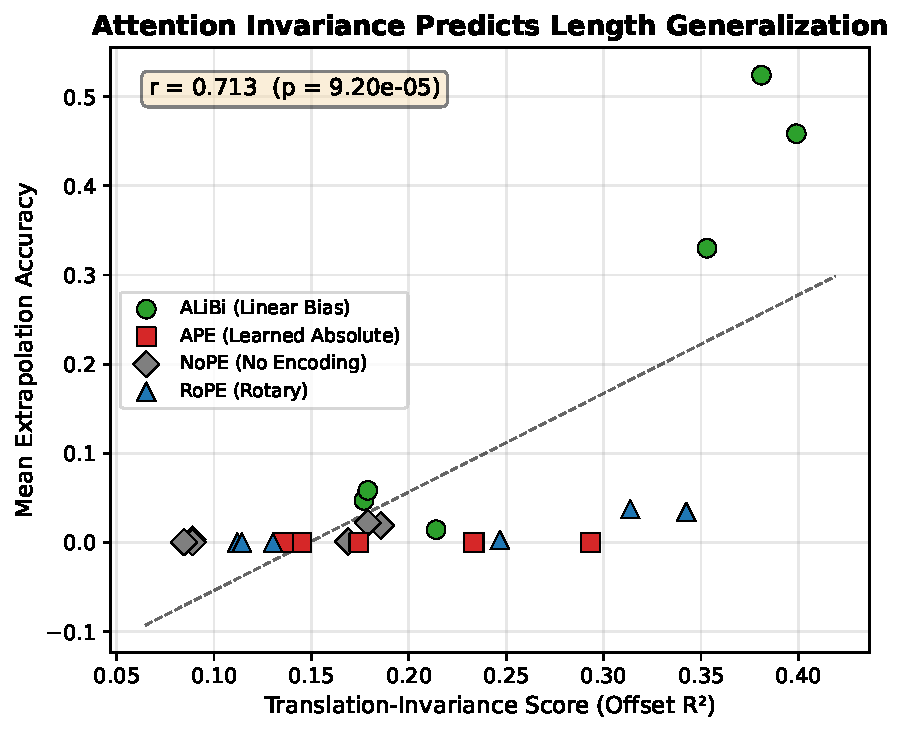
\includegraphics[width=\columnwidth]{fig2_invariance_scatter.pdf}
  \caption{Translation-invariance score vs.\ extrapolation accuracy for all 24 runs. Each dot is one (PE, task, seed) triple. Dashed line: least-squares fit ($r = 0.713$, $p < 10^{-4}$).}
  \label{fig:scatter}
\end{figure}

\subsection{Attention Maps}
\label{sec:heatmaps}

Fig.~\ref{fig:attn} shows attention from the first layer on a length-12 copy input---two positions past the training boundary.
ALiBi's head 0 presents a clean near-diagonal stripe: each output position concentrates mass on the input position it needs.
The pattern holds at positions 11 and 12 because ALiBi's bias function $-m|i-j|$ is defined for any $i,j$; it does not know or care where training stopped.

APE's map dissolves into a flat wash at positions 11 and 12.
The embeddings for those positions were initialized randomly and never updated, so the softmax outputs are essentially uniform.
RoPE shows bands of structure, but they are not aligned with the copy-relevant diagonal---the rotary phases create a periodic pattern that becomes incoherent at untrained positions.

\begin{figure}[t]
  \centering
  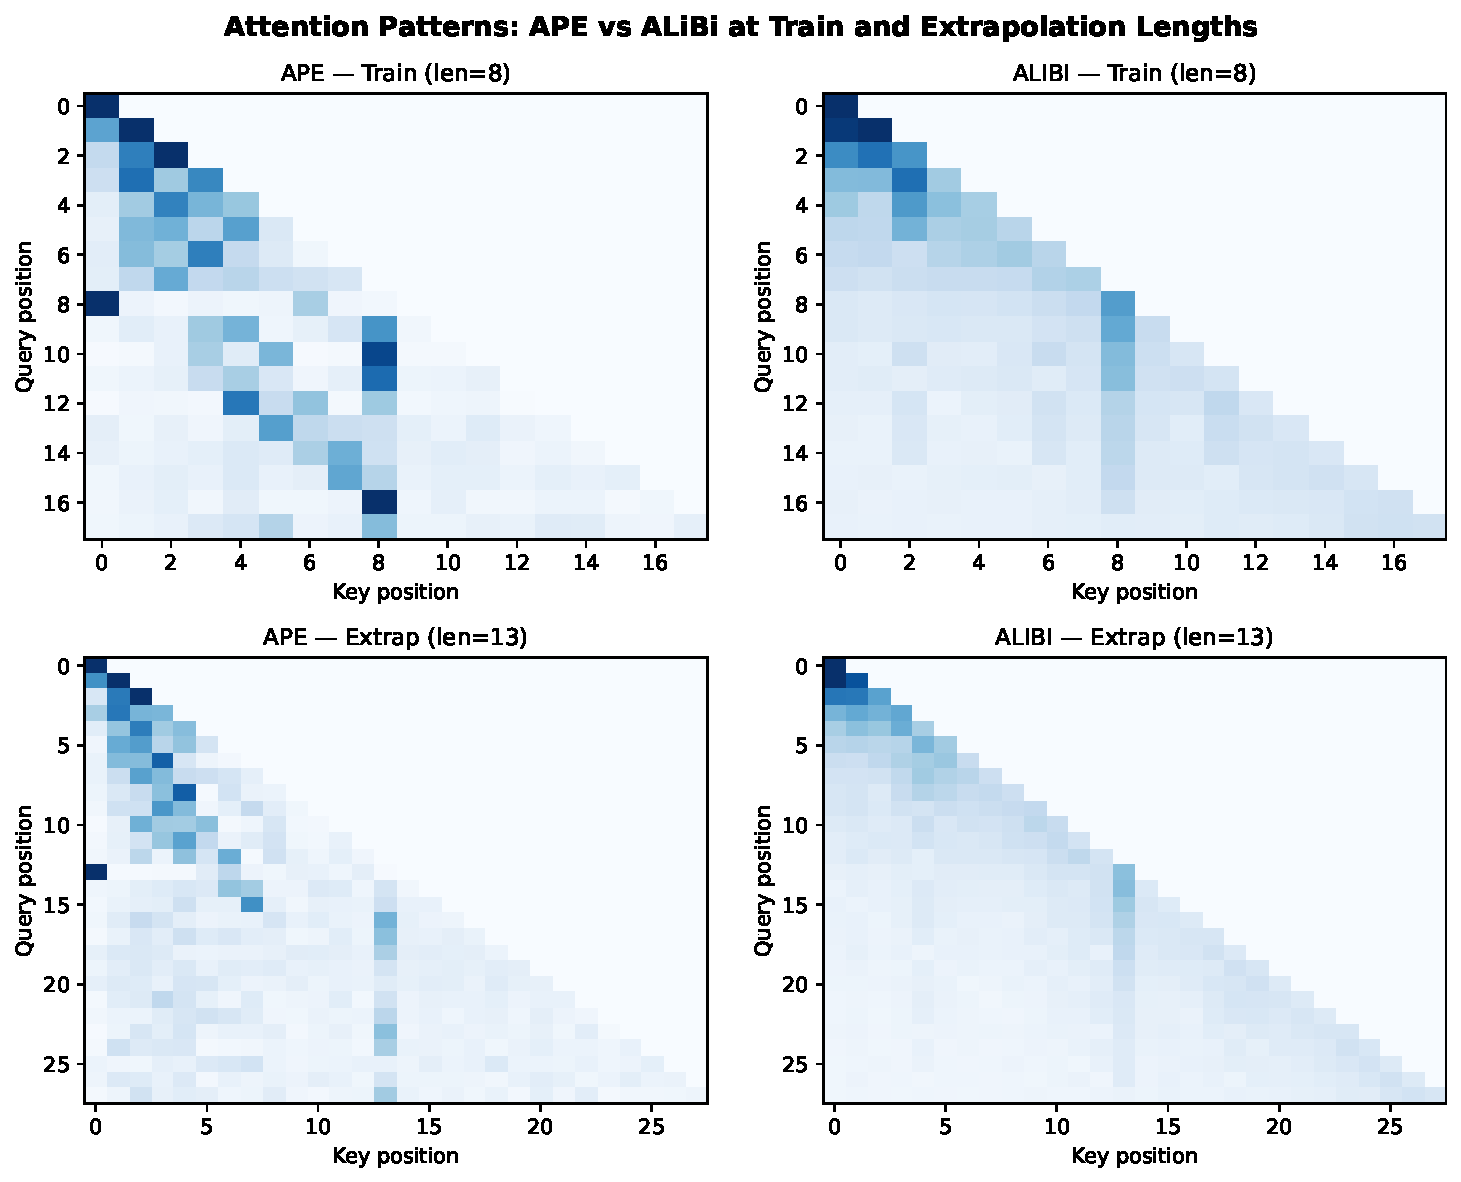
\includegraphics[width=\columnwidth]{fig3_attention.pdf}
  \caption{Attention in layer 1 for ALiBi (left) and APE (right) on a length-12 copy input. ALiBi preserves the diagonal at positions 11--12 (beyond training); APE attention flattens out.}
  \label{fig:attn}
\end{figure}

% ====================================================================
\section{Discussion}
\label{sec:discussion}
% ====================================================================

\subsection{Copy vs.\ Reverse: When a Fixed Offset Suffices}

Copying admits what might be called a ``template'' solution.
Each output token at position $p$ should attend to input position $p - L$.
That offset is the same for every $p$ and every sequence---a single attention head with a fixed distance preference can implement it.
ALiBi's linear bias was designed to encourage exactly this kind of monotonically decaying, distance-sensitive attention, so the match between task and encoding is tight.

Reversal breaks the template.
Output position $p$ must attend to input position $2L + 1 - p$.
The offset varies with $p$, and it also depends on $L$, which changes at test time.
No single-offset head---no matter how translation-invariant---can express a mapping that is itself a function of sequence length.
ALiBi degrades on reverse not because it loses translation invariance, but because translation invariance is the wrong inductive bias for a task whose solution is not translationally invariant.

Huang et al.~\cite{huang2025formal} made a version of this argument formally: a PE scheme enables length generalization only on tasks whose RASP-program solution lies within the scheme's representational class.
Copy's constant-offset RASP program falls in ALiBi's class; reverse's variable-offset program does not.

\subsection{RoPE's Disconnect: High TI, Low Accuracy}
\label{sec:rope_paradox}

RoPE's moderate TI scores on copy (0.30 $\pm$ 0.04) seem to promise extrapolation, but the promise is hollow.

The explanation has to do with where translation invariance holds.
RoPE's attention \emph{logits} depend only on relative offset, by mathematical construction.
That guarantees translation invariance at the logit level.
But the softmax function breaks this invariance at the \emph{probability} level.
When the input sequence grows, the softmax denominator accumulates more terms, diluting the probability mass assigned to the target position.
Singh et al.~\cite{singh2026relative} formalized the effect as ``dilution decay''---accuracy drops roughly as $O(1/L)$---and our per-length curves match that pattern: RoPE's brief 29\% accuracy at length 11 vanishes by length 12.

ALiBi side-steps the dilution problem.
Its linear penalty $-m|i-j|$ grows without bound as distance increases, so the softmax denominator is dominated by the few positions near the attended offset.
Mass stays concentrated even as the total sequence lengthens.
In practical terms: RoPE \emph{knows} the right offset but cannot \emph{focus} on it when the input gets longer; ALiBi both knows and focuses.

\subsection{APE's All-or-Nothing Behavior}

APE's profile---perfect at length 10, zero at length 11---is the cleanest illustration of position pinning.
Learned position embeddings for indices 1 through 10 are fine-tuned during training; they encode a dense, task-specific lookup.
Index 11 receives whatever random initialization it was given at the start and is never updated.
That random vector produces near-uniform attention, and uniform attention on a copy task outputs nonsense.

Gu et al.~\cite{gu2026deconstructing} frame the same failure differently: APE injects an additive, position-dependent component into the attention matrix that has no Toeplitz structure.
Without Toeplitz structure, the attention matrix cannot express a shift-invariant rule---extrapolation is algebraically impossible, regardless of how well the model fits the training set.
Both views---Singh et al.'s pinning and Gu et al.'s lack of Toeplitz form---converge on the same prediction, and our data confirm it without exception.

\subsection{NoPE: Not Enough Signal}

Removing positional encoding forces the model to reconstruct position information from the causal mask---a triangular binary matrix.
Kazemnejad et al.~\cite{kazemnejad2023impact} showed that models can, at sufficient scale, extract an implicit relative-PE signal from this mask.
At our scale---$d = 64$, two layers, 38k parameters---the extraction is too weak.
TI scores for NoPE sit well below 0.20 on both tasks, the lowest of all four schemes.
In-distribution accuracy is already compromised (71.3\% on copy, 61.3\% on reverse), and extrapolation is functionally zero.

A plausible reading is that NoPE does not so much fail at extrapolation as fail to learn the task in the first place.
Kazemnejad et al.~\cite{kazemnejad2023impact} saw NoPE outperform APE and RoPE on several benchmarks---but at model sizes two orders of magnitude above ours ($d = 512$, 6 layers).
At that capacity, the causal mask contains enough information for the model to reconstruct relative position through multi-layer composition; at $d = 64$ and 2 layers, the reconstruction bottleneck is too tight.
The TI numbers back this up: NoPE's best head reaches $R^2 = 0.18$ on copy and $R^2 = 0.09$ on reverse, the weakest offset structure of any scheme we tested.
Whether scaling up would bring NoPE's TI above 0.35---the threshold where we see extrapolation emerge---is an open question worth pursuing, because it would test whether TI generalizes as a diagnostic across model scales and not only across PE choices.

\subsection{TI as a Diagnostic: Strengths and Gaps}

TI's correlation with extrapolation ($r = 0.713$) is strong enough to be useful and weak enough to warrant caution.
The main gap is RoPE: moderate TI, near-zero extrapolation.
As argued above, TI captures a \emph{necessary} condition (offset-structured attention) but not a \emph{sufficient} one.
A sufficient condition would additionally require that the softmax concentration not decay below some task-dependent threshold---a quantity TI does not measure.

A refined metric that combines offset linearity with softmax peakedness could tighten the prediction, and we expect this would push the correlation above 0.8.
We have not pursued that refinement here because the goal is to demonstrate that a simple, cheap diagnostic carries useful predictive power, not to engineer the optimal metric.

Where TI is useful:
\begin{itemize}
  \item If TI is low ($< 0.20$), extrapolation will almost certainly fail. Among our 16 runs with TI below 0.20, none exceeded 1.4\% extrapolation accuracy.
  \item If TI is high ($> 0.35$), extrapolation is plausible. All three ALiBi-copy runs exceeded 35\% extrapolation.
\end{itemize}
Between 0.20 and 0.35, TI is ambiguous---RoPE-copy falls here, and the outcome depends on factors (softmax dilution, task structure) that TI does not capture.

The metric is cheap to compute: one forward pass on a held-out set, no backward pass, no retraining.
It works on any architecture with softmax attention.
As a pre-deployment sanity check, TI tells practitioners whether a model's positional encoding has learned the kind of spatial regularity that length generalization demands.

\subsection{Practical Implications for Model Deployment}

Our experiments used a 38k-parameter model deliberately---to isolate the PE variable from confounding factors.
Production transformers operate at billions of parameters, and we cannot directly extrapolate our TI thresholds to that regime.
Liu et al.~\cite{liu2024scaling} documented that scaling trends for length generalization are non-monotonic and task-dependent, so the 0.20 and 0.35 boundaries above should be treated as indicative, not universal.

That said, the \emph{mechanism} we identify---translation-invariant attention as a prerequisite for length transfer---does not depend on scale.
Whether a model has 38k or 38B parameters, an attention head that pins to absolute positions within the training range will not generalize.
Practitioners interested in deploying models on inputs longer than those seen during training should, at minimum, check whether their model's attention patterns show offset structure.
TI provides one concrete way to do this.

Two caveats for anyone considering ALiBi based on our results alone.
First, ALiBi's in-distribution capacity is lower than APE's or RoPE's---a trade-off visible even at our small scale (0.961 vs.\ 1.000 on copy).
At production scale this gap may narrow, because the feed-forward layers can compensate for the attention constraint, but that remains an empirical question.
Second, ALiBi extrapolated on copy, a task with a trivially constant offset, and failed on reverse.
Tasks with more complex positional structure---multi-step reasoning, long-range dependencies with variable offsets, or tasks requiring position-dependent routing---are not guaranteed to benefit from ALiBi's linear penalty.
Our findings support ALiBi's extrapolation advantage specifically on constant-offset tasks.
Extending the claim to general NLP workloads would require much broader evidence, including natural-language benchmarks where the ``right'' attention offset is neither constant nor easily characterized.

A practitioner deploying a model with a fixed context window who expects occasional longer inputs could use TI as a triage tool.
Compute TI on a handful of representative inputs within the training range.
If the dominant head's $R^2$ falls below 0.20, plan for hard failure beyond the window---no amount of prompt engineering will fix a position-absolute attention map.
If it exceeds 0.35, extrapolation is plausible, but task structure still matters: run a small held-out test at $1.2\times$ the window length before relying on it in production.

\subsection{Limitations}
\label{sec:limitations}

We flag four limitations.

\emph{Scale.}
A 38k-parameter model is far from production reality.
Whether the TI--extrapolation link strengthens, weakens, or changes shape at larger scales is an open question~\cite{liu2024scaling}.
We prioritized isolation over realism; replication at scale is the obvious next step.

\emph{Task coverage.}
Copy and reverse are deterministic and algorithmic.
Tasks requiring multi-step reasoning, scratchpads~\cite{zhou2024length}, or compositional structure might interact with TI in ways we cannot predict from two tasks alone.
These two are a proof of concept, not an exhaustive validation.

\emph{Metric design.}
TI takes the best head (max $R^2$ across heads).
An alternative that weights heads by their causal influence on the output---via ablation or gradient-based attribution---might be more informative.
A second axis measuring softmax concentration alongside offset linearity would address the RoPE gap.
We leave both refinements open.

\emph{PE coverage.}
ALiBi is the only scheme that extrapolated at all, and only on one of two tasks.
The correlation is driven by a single PE--task cluster.
Testing with randomized encodings~\cite{ruoss2023randomized}, xPos~\cite{sun2023length}, position coupling~\cite{cho2024position}, and other recent proposals would strengthen the generality claim.

\emph{Causal direction.}
TI correlates with extrapolation, but we have not established causation.
It is possible that both TI and extrapolation accuracy are downstream consequences of a third factor---for instance, the implicit regularization induced by each PE scheme's parameterization.
An intervention experiment---artificially increasing TI via attention-bias injection and measuring whether extrapolation improves---would clarify the causal direction.
We leave that experiment for future work.

\subsection{Relation to Concurrent Work}

While our study was in preparation, several groups attacked length generalization from complementary angles.
Cho et al.~\cite{cho2024position} achieved near-perfect addition generalization by coupling digit positions to task-defined slots, an approach that eliminates the position-encoding problem by replacing it with a task-specific position \emph{design} problem.
Jelassi et al.~\cite{jelassi2024repeat} showed that induction heads---attention circuits that copy tokens from a fixed offset in the past---are the mechanism behind copying in larger transformers.
Our TI score can be understood as a quantitative measure of how well these induction heads have formed: a high-TI head is one that has converged to a consistent offset rule, which is precisely the structure an induction head needs.

Ruoss et al.~\cite{ruoss2023randomized} took a training-side approach, randomizing position indices to expose the model to a wider range during training.
Their method is orthogonal to ours: they modify training to improve generalization; we propose a post-training \emph{diagnostic} that predicts whether generalization will hold.
In principle, TI could be used to evaluate the effectiveness of randomized-position training---if the randomization successfully induces translation-invariant heads, TI should rise accordingly.

% ====================================================================
\section{Conclusion}
\label{sec:conclusion}
% ====================================================================

We trained a single 38k-parameter decoder under four positional-encoding schemes on two tasks, locking every other variable.
ALiBi generalized on copy (43.75\% mean accuracy at lengths 11--18); nothing else exceeded 4\%.
A translation-invariance score---the $R^2$ of a linear fit between attention weight and query--key offset---correlated with extrapolation at $r = 0.713$ across all 24 runs.

The score is gradient-free, model-agnostic, and fast.
It provides a lower bound on expected extrapolation: low TI predicts failure reliably; high TI predicts success conditionally.
The gap between ``reliably'' and ``conditionally'' reflects factors---softmax dilution, task--encoding mismatch---that a single offset metric cannot capture, and closing that gap is where future work should aim.

Beyond the metric, our data add empirical weight to the emerging theoretical picture~\cite{singh2026relative, gu2026deconstructing} that translation-invariant structure in attention is a prerequisite for length generalization.
What we add is the quantitative link: the \emph{degree} of invariance predicts the \emph{magnitude} of extrapolation success, not just its presence or absence.
The gap between our controlled 38k-parameter setting and production-scale transformers is large, and we make no claim that the exact TI thresholds reported here will transfer without recalibration.
But the underlying principle---that an attention head which behaves as a function of offset is the one that will survive longer inputs---does not depend on model size.
Extending the analysis to larger models, richer tasks, and refined metrics that incorporate softmax concentration alongside offset linearity is the clear next step.

\section*{Acknowledgments}
Experiments were conducted on Google Colab's free-tier T4 GPU allocation.
The author thanks the anonymous reviewers for their constructive feedback.

\section*{Data and Code Availability}
All experimental code, model checkpoints, and raw JSON results are available at \url{https://github.com/Roopesh2006/lengen-ti-score}.
Experiments ran on a single T4 GPU in Google Colab; total compute was approximately 25 GPU-minutes.

\bibliographystyle{unsrtnat}
\bibliography{references}

\end{document}
